% !TeX program = pdflatex
\documentclass[tikz,border=8pt]{standalone}
\usepackage{tikz}
\usetikzlibrary{intersections,positioning}
\definecolor{FigureBlue}{HTML}{2563EB}
\definecolor{FigureOrange}{HTML}{EA580C}
\begin{document}
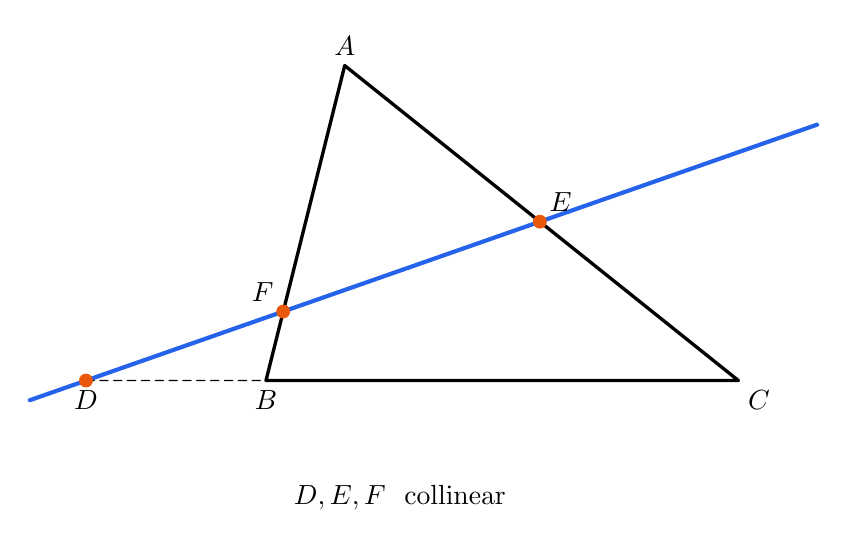
\begin{tikzpicture}[line cap=round,line join=round]
  \coordinate (A) at (1,4);\coordinate (B) at (0,0);\coordinate (C) at (6,0);
  \coordinate (X) at (-3,-.25);\coordinate (Y) at (7,3.25);
  \path[name path=AB] (A)--(B);\path[name path=CA] (C)--(A);
  \path[name path=BCext] (-3,0)--(7,0);\path[name path=transversal] (X)--(Y);
  \path[name intersections={of=transversal and BCext,by=D}];
  \path[name intersections={of=transversal and CA,by=E}];
  \path[name intersections={of=transversal and AB,by=F}];
  \draw[line width=1.2pt] (A)--(B)--(C)--cycle;
  \draw[densely dashed] (D)--(B);
  \draw[FigureBlue,line width=1.5pt] (X)--(Y);
  \foreach \P in {D,E,F}{\fill[FigureOrange] (\P) circle (2.5pt);}
  \node[above] at (A) {$A$};\node[below] at (B) {$B$};\node[below right] at (C) {$C$};
  \node[below] at (D) {$D$};\node[above right] at (E) {$E$};\node[above left] at (F) {$F$};
  \node[below=12mm] at (1.7,0) {$D,E,F\ \hbox{ collinear}$};
\end{tikzpicture}
\end{document}
